% \meutodo{
%   Variação gradual de parâmetros para identificar o que causa perdas/ganhos
% }

%%%%%%%%%%%%%%%%%%%%%%%%%%%%%%%%%%%%%%%%%%%%%%%%%%%%%%%%%%%%%%%%%%%%%%%%%%%%%%%%
\section{Considerações Iniciais}

Este capítulo apresenta os resultados encontrados ao aplicar os métodos de quantização de imagens no \textit{pipeline} implementado. Para cada experimento realizado são descritos: a base de imagens; o protocolo utilizado; os resultados encontrados e a sua relevância.
%Vale ressaltar que os experimentos são relacionados à quantização de imagens, realizada antes da etapa de extração de características.
Os resultados devem refletir melhoras nas etapas subsequentes, como uma melhor acurácia na etapa de classificação ou a redução do tempo de processamento.

%%%%%%%%%%%%%%%%%%%%%%%%%%%%%%%%%%%%%%%%%%%%%%%%%%%%%%%%%%%%%%%%%%%%%%%%%%%%%%%%
\section{Experimentos}

O objetivo desta seção é mostrar os efeitos da etapa de quantização e como ela pode ser utilizada para reduzir a dimensionalidade do espaço de características ou a complexidade em etapas posteriores do \textit{pipeline} de classificação. A Figura~\ref{fig:quant:flowResult} demonstra o fluxo das operações, juntamente com os métodos utilizados nos experimentos.

\begin{figure}[!htbp]
  \begin{center}
    \centering
    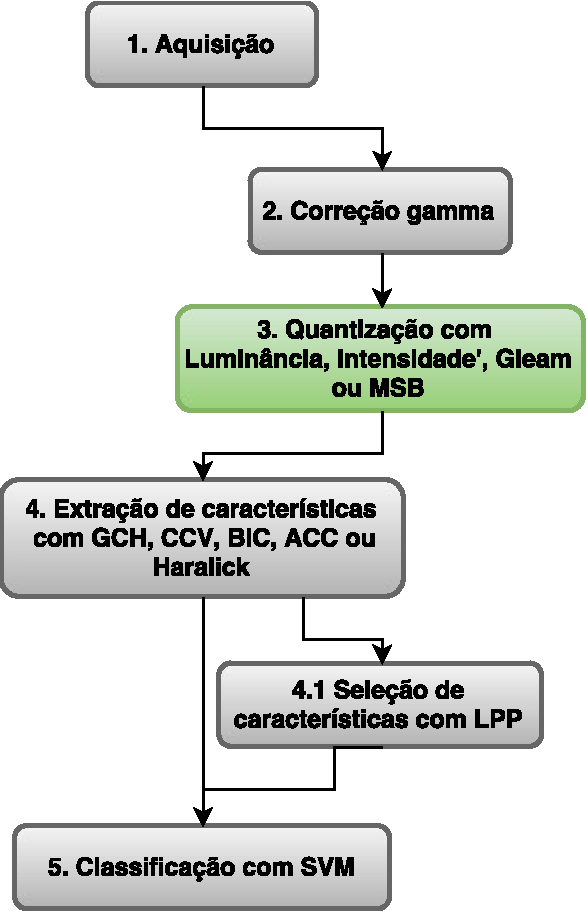
\includegraphics[width=0.4\linewidth]{\detokenize{figuras/quantizacao/quantizationResult.pdf}}
  \end{center}
  \caption[Essa figura demonstra o fluxo das operações e os métodos utilizados nos experimentos. Após a aquisição da imagem, ela é convertida para escala de cinza e seus níveis de cor são reduzidos de acordo com um parâmetro da quantização (i.e.\ número de cores). Dependendo do método, a correção \emph{gamma} é realizada. A imagem quantizada serve então como entrada para um método de extração de características e posteriormente é classificada com \emph{SVM}. Uma das etapas de experimentos prevê também a concatenação de todos os vetores extraídos e a seleção das características com \emph{LPP} antes da classificação.]{Essa figura demonstra o fluxo das operações e os métodos utilizados nos experimentos. Após a aquisição da imagem, ela é convertida para escala de cinza e seus níveis de cor são reduzidos de acordo com um parâmetro da quantização (i.e.\ número de cores). Dependendo do método, a correção \emph{gamma} é realizada. A imagem quantizada serve então como entrada para um método de extração de características e posteriormente é classificada com \emph{SVM}. Uma das etapas de experimentos prevê também a concatenação de todos os vetores extraídos e a seleção das características com \emph{LPP} antes da classificação. \\ \textit{Fonte:~Elaborado pela autora.}}
  \label{fig:quant:flowResult}
\end{figure}

Inicialmente, as imagens foram quantizadas em 256, 128, 64, 32 e 16 cores. Dependendo do método de conversão para a escala de cinza, a correção \textit{gamma} é realizada (ver Seção \ref{sec:quantizacao}). Após, suas características são extraídas e duas etapas distintas de experimentos são realizadas:

\begin{enumerate}
  \item Experimentos utilizando um método de extração de características seguido pela classificação (sem posterior seleção de características);
  \item Experimentos utilizando o vetor resultante da concatenação de todos os métodos de extração, seguido pela classificação com e sem a seleção de características.
\end{enumerate}

%%%%%%%%%%%%%%%%%%%%%%%%%%%%%%%%%%%%%%%%%%%%%%%%%%%%%%%%%%%%%%%%%%%%%%%%%%%%%%%%
\subsection{Base de Imagens}

Três bases de imagens, exemplificadas na Figura~\ref{fig:quant:bases}, foram utilizadas nestes experimentos de quantização:
\begin{itemize}
\item[] \textbf{Corel-1000} \cite{Wang2001}: consiste em dez classes balanceadas de imagens naturais, com algumas classes bem definidas e algumas não;
\item[] \textbf{Caltech101-600} \cite{Fei-Fei2007}: contém fotos e desenhos. Dessa base, foi utilizado um conjunto de seis classes balanceadas: aviões, bonsais, candelabros, tartarugas, motocicletas e relógios;
\item[] \textbf{Produce} \cite{Rocha2010}: também conhecido como base de vegetais e frutas tropicais. Composta por imagens com um fundo similar mas mudanças representativas na iluminação, no número de objetos e na escala. Apesar da oclusão parcial de objetos ser observada, essa classe possui dados bem comportados.
\end{itemize}

\begin{figure}[!htbp]
  \begin{center}
    \subfloat[Base de imagens Caltech101]{
      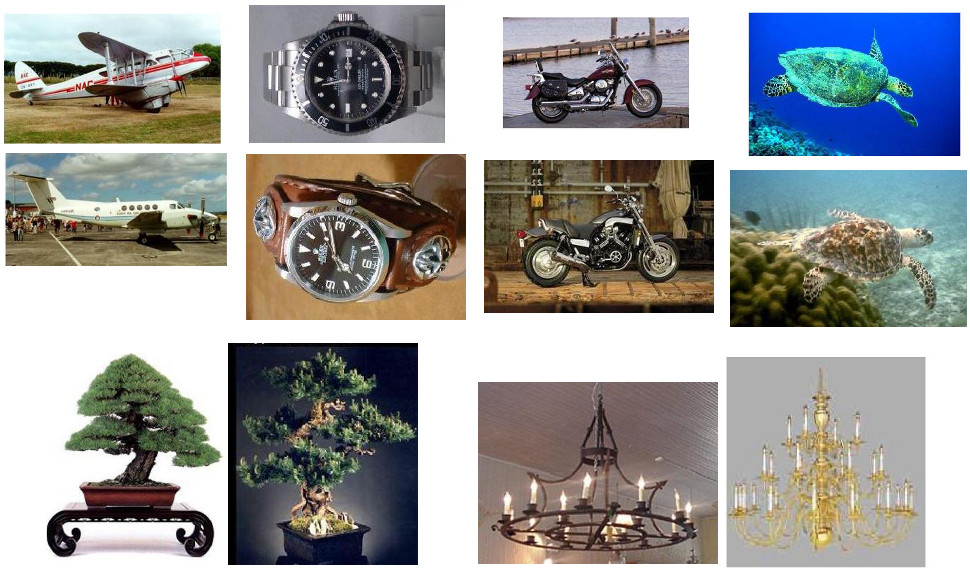
\includegraphics[width=\linewidth]{\detokenize{figuras/quantizacao/fig_Caltech101_dataset.jpg}}
    }
    \newline
    \subfloat[Base de imagens Corel-1000]{
      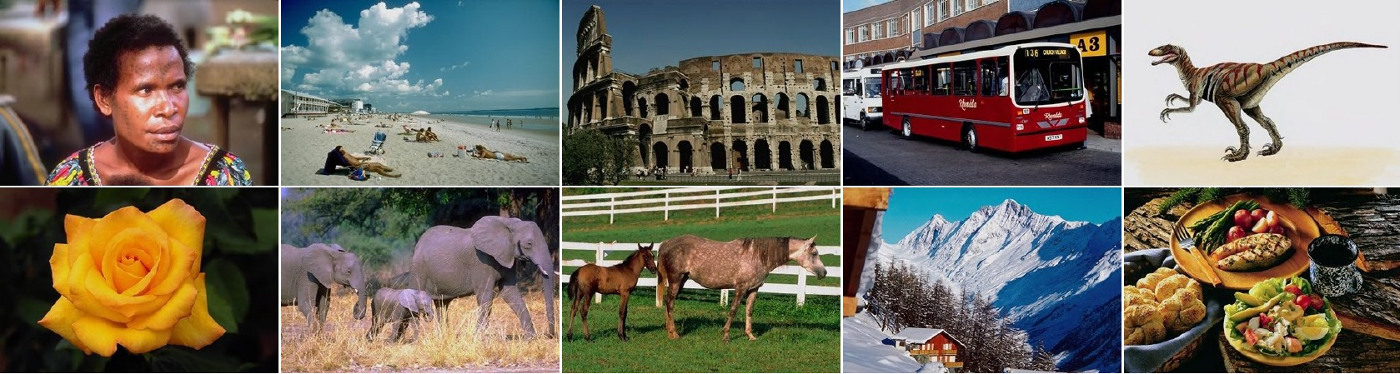
\includegraphics[width=\linewidth]{\detokenize{figuras/quantizacao/fig_COREL_dataset.jpg}}
    }
    \newline
    \subfloat[Base de imagens Produce]{
      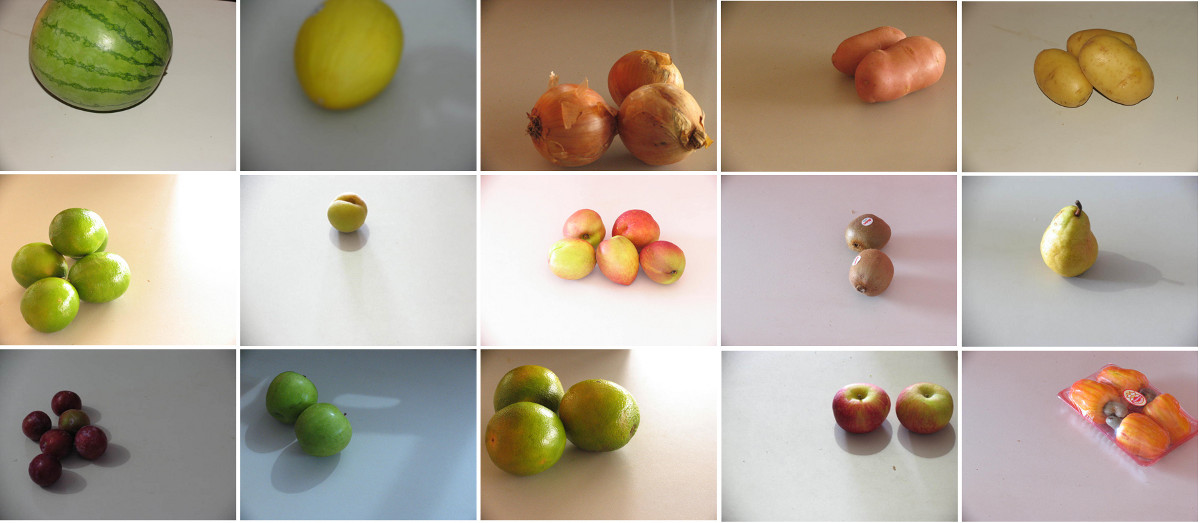
\includegraphics[width=\linewidth]{\detokenize{figuras/quantizacao/fig_Produce_dataset.jpg}}
    }
  \end{center}
  \caption[Bases de imagens utilizadas para os experimentos de quantização.]{Bases de imagens utilizadas para os experimentos de quantização. \\ \textit{Fonte:~\cite{Ponti2016}.}}
  \label{fig:quant:bases}
\end{figure}

Considerando que estes experimentos possuem foco na redução na dimensionalidade, para evitar o problema do desbalanceamento, as bases \textit{Produce} e \textit{Caltech} foram modificadas. Dessa forma, as classes disponíveis foram balanceadas ao remover imagens das classes majoritárias.

%%%%%%%%%%%%%%%%%%%%%%%%%%%%%%%%%%%%%%%%%%%%%%%%%%%%%%%%%%%%%%%%%%%%%%%%%%%%%%%%
\subsection{Protocolo}

Os experimentos foram realizados com uma validação cruzada de \textit{10-fold}. Considerando que as bases estão balanceadas e que a seleção de exemplos para a validação cruzada é estratificada, a medida estatística de \textit{acurácia} foi utilizada para avaliar a performance da classificação. O seguinte protocolo foi seguido para a obtenção dos resultados:

\begin{enumerate}
\item \textbf{Quantização}: com os métodos \emph{Intensidade'}, \emph{Gleam}, \emph{Luminância'} e MSB.
\item \textbf{Extração de características}: utilizando os métodos -- e parâmetros escolhidos com base nas recomendações dos artigos que proporam tais métodos -- a seguir:
  \begin{itemize}
    \item \textit{Auto Color Correlogram} (ACC): a métrica de distância utilizada entre os pixels $p(x,y)$ e $q(s,t)$ é a tabuleiro de xadrez $D_8(p,q) = Max(|x-s| + d, |y-t| + d)$ para quatro distâncias $d =$ 1, 3, 5 e 7;
    \item \textit{Border-Interior Classification} (BIC): com uma vizinhança de quatro pixels;
    \item \textit{Color Coherence Vector} (CCV): adotando um valor de $\mathit{threshold} = 25$ para a classificação dos pixels entre coerentes e incoerentes;
    \item Haralick-6: o pixel vizinho para o qual iniciar a computar a matriz de co-ocorrência foi o pixel à direita.
  \end{itemize}
\item \textbf{Redução da dimensionalidade}: a projeção utilizando \textit{Locality Preserving Projections} (LPP) foi realizada com o parâmetro $k =$ 128, 64, 32 e 16 dimensões e 10 vizinhos. Esse parâmetro foi determinado empiricamente e não influencia consideravelmente a acurácia.
\item \textbf{Classificação}: realizada com o classificador \textit{Support Vector Machines} (SVM). Os parâmetros para essa etapa foram encontrados utilizando uma \textit{grid search} no conjunto de treinamento.
\end{enumerate}

%%%%%%%%%%%%%%%%%%%%%%%%%%%%%%%%%%%%%%%%%%%%%%%%%%%%%%%%%%%%%%%%%%%%%%%%%%%%%%%%
\section{Resultados e Discussão}

A Figura \ref{fig:quant:results} ilustra a acurácia média para o primeiro conjunto de experimentos: para cada combinação de base de dados e método de extração, são demonstrados seis resultados de acurácia correspondentes à quantização para 256, 128, 64, 32, 16 e 8 cores. Com base nessa figura é possível identificar que o método para obter a imagem quantizada tem um impacto significativo na acurácia da classificação. Além disso, a redução de 256 para um menor número de cores normalmente manteve as acurácias e em alguns casos resultou em uma ligeira melhora, especialmente para os níveis de 128 e 64.

\begin{figure}[!htbp]
  \begin{center}
    \centering
    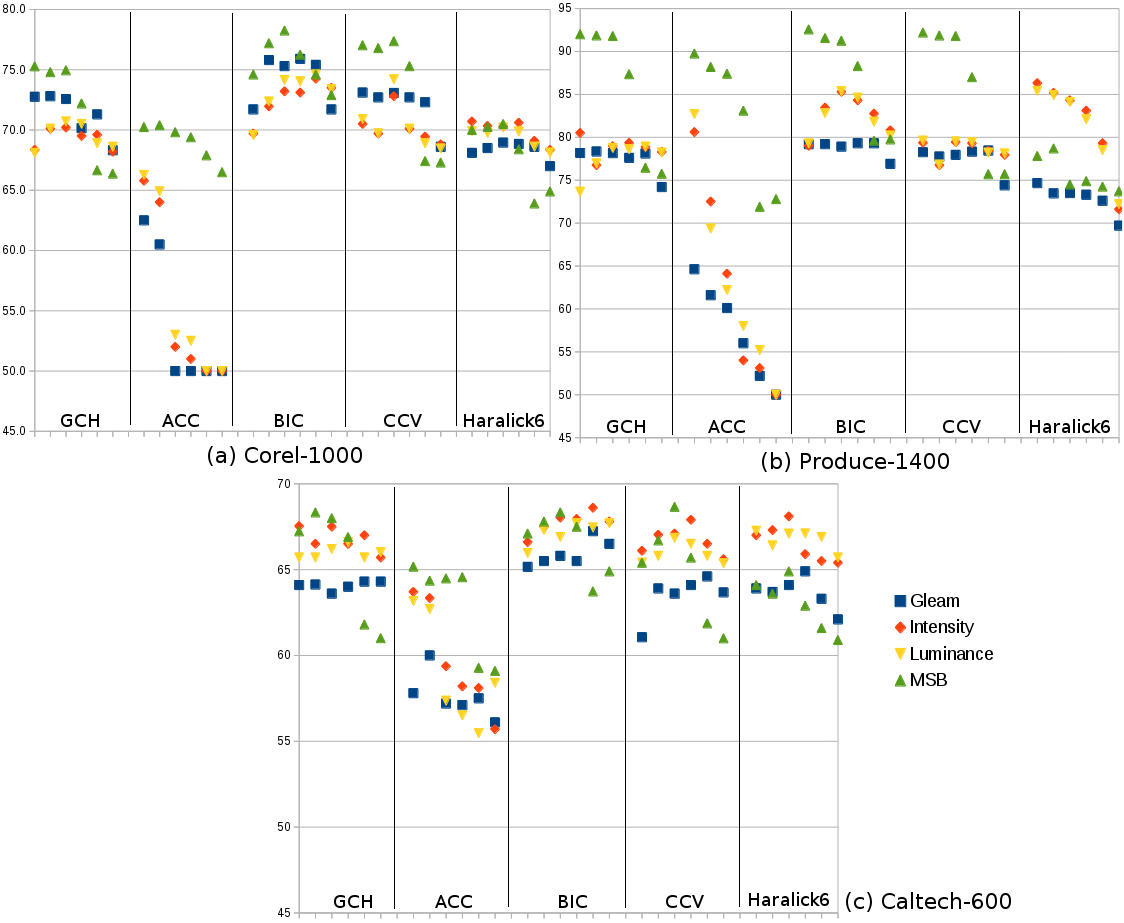
\includegraphics[width=\linewidth]{\detokenize{figuras/quantizacao/fig_results_individual.png}}
  \end{center}
  \caption[Resultados para Corel (a), Produce (b) e Caltech (c), utilizando todos os métodos de quantização. Para cada método de extração de características a acurácia é resultante da sua aplicação utilizando 256, 128, 64, 32, 16 e 8 cores, da esquerda para a direita.]{Resultados para Corel(a), Produce(b) e Caltech(c), com todos os métodos de quantização. Para cada método de extração de características a acurácia é resultante da sua aplicação utilizando 256, 128, 64, 32, 16 e 8 cores, da esquerda para a direita. \\ \textit{Fonte:~\cite{Ponti2016}.}}
  \label{fig:quant:results}
\end{figure}

Considerando que a utilização de apenas 16 e 8 cores resultou em uma acurácia muito inferior, o restante dos resultados utilizam 256, 128, 64 e 32 cores. A partir dessa análise geral, uma análise mais específica foi realizada com a combinação dos métodos BIC e MSB; e Haralick e \emph{Luminância'}. O teste estatístico ANOVA foi realizado para comparar as acurácias dos experimentos das Figuras \ref{fig:quant:boxplotBIC} e \ref{fig:quant:boxplotHaralick}. Para identificar se algum método obteve uma diferença significativa no valor de acurácia, foi utilizado o teste \sigla{HSD}{\textit{Honest Significant Difference}} de Tukey. Um nível de significância de $\alpha = 0.01$ foi utilizado. Por conta disso, os \textit{boxplots} em cinza correspondem aos dados com diferença estatística relevante quando comparados com a acurácia de 256 cores, obtendo um $p < 0.01$.

% O boxplot para 256, 128, 64 e 32 cores com os métodos \emph{BIC} e MSB está demonstrado na Figura \ref{fig:quant:boxplotBIC}.

De acordo com o teste estatístico representado na Figura \ref{fig:quant:boxplotBIC}, utilizar características de cor (extraídas com o método BIC) e níveis de quantização providos pelo método MSB demonstrou resultados melhores do que o \textit{baseline} de 256 cores para as bases Corel (128, 64 e 32 cores) e Caltech (64 cores). O único resultado que piorou significativamente foi para 32 cores da base de imagens \textit{Produce}. Portanto, converter as imagens para a escala de cinza e reduzir os 256 possíveis valores para apenas 64 provou uma boa escolha de processamento anterior a extração de características. Menores valores podem degradar os resultados em características de textura, como mostrado na Figura \ref{fig:quant:boxplotHaralick}.

\begin{figure}[!htbp]
  \begin{center}
    \centering
    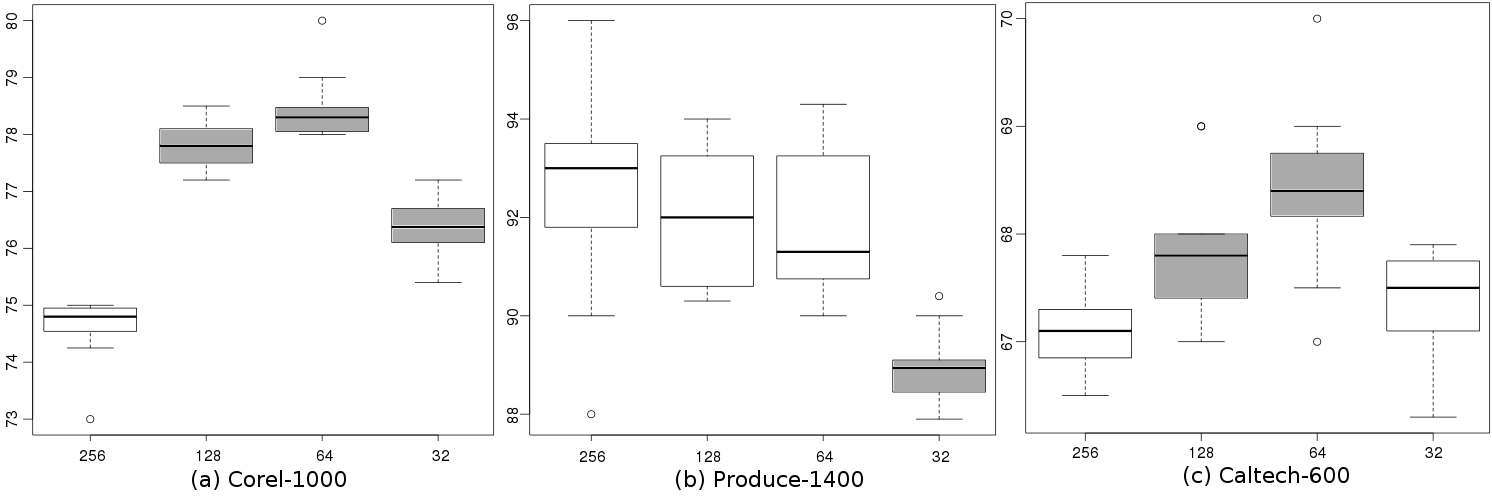
\includegraphics[width=\linewidth]{\detokenize{figuras/quantizacao/fig_results_individual_boxplotBIC.png}}
  \end{center}
  \caption[Resultados de acurácia média da classificação utilizando o método de quantização MSB considerando 256, 128, 64 e 32 cores com o método de extração de características BIC. Os boxplots em cinza correspondem às significâncias estatísticas com $p < 0.01$ quando comparado à acurácia de 256 cores.]{Acurácia média da classificação utilizando o método de quantização MSB considerando 256, 128, 64 e 32 cores com o método de xtração de características BIC. Os boxplots em cinza correspondem às significâncias estatísticas com $p < 0.01$ quando comparado à acurácia de 256 cores. \\ \textit{Fonte:~\cite{Ponti2016}.}}
  \label{fig:quant:boxplotBIC}
\end{figure}

\begin{figure}[!htbp]
  \begin{center}
    \centering
    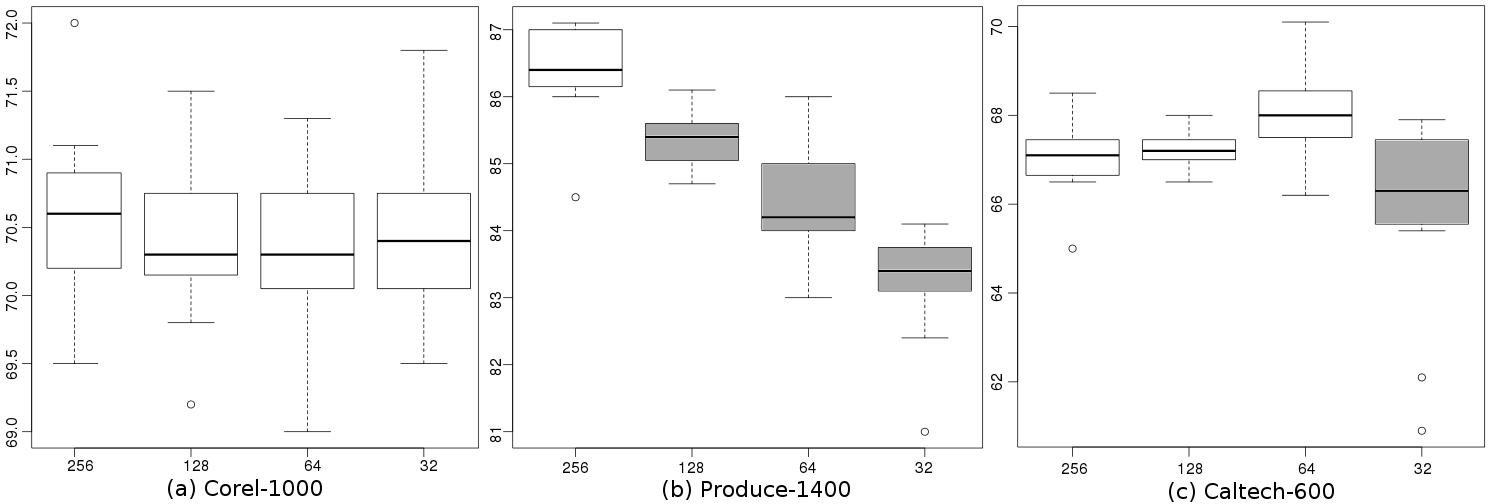
\includegraphics[width=\linewidth]{\detokenize{figuras/quantizacao/fig_results_individual_boxplotHaralick.png}}
  \end{center}
  \caption[Acurácia média da classificação após a utilização do método de quantização \emph{Luminância'} considerando 256, 128, 64 e 32 cores com o descritor Haralick. Os boxplots em cinza correspondem às significâncias estatísticas com $p < 0.01$ quando comparado à acurácia de 256 cores.]{Acurácia média da classificação após a utilização do método de quantização \emph{Luminância'} considerando 256, 128, 64 e 32 cores com o descritor Haralick. Os boxplots em cinza correspondem às significâncias estatísticas com $p < 0.01$ quando comparado à acurácia de 256 cores. \\ \textit{Fonte:~\cite{Ponti2016}.}}
  \label{fig:quant:boxplotHaralick}
\end{figure}

Uma outra comparação importante é entre a redução de dimensionalidade obtida com métodos de quantização versus o método LPP. A redução de dimensionalidade obtida com os métodos MSB, BIC e LPP está ilustrada na Figura \ref{fig:quant:boxplotMSBLPP}. A imagem de entrada foi convertida para escala de cinza com o método MSB em 256 cores. Essa imagem foi dada como entrada para o método de extração de características BIC, que resultou em um vetor dado como entrada para o LPP. Esse último passo teve o objetivo de produzir versões reduzidas desse vetor para 256, 128 e 64 dimensões. As acurácias obtidas foram então comparadas com a classificação dos vetores reduzidos apenas pela quantização. Como a comparação foi feita em pares, foram realizados testes t de Student sobre a suposição de dois exemplos independentes com variâncias desiguais e um nível de significância de $0.01$. O método de quantização obteve valores de acurácia menores à utilização do LPP em três experimentos: 256 cores com a base \textit{Corel} e com 256 e 64 na base \textit{Produce}. Para a base \textit{Caltech} a quantização foi melhor com 256 e 128 dimensões. O restante dos experimentos não apresentaram diferença estatística relevante. Apesar da perda de acurácia em alguns casos, é importante notar que -- se utilizado um número de cores correto -- é possível manter ou até mesmo melhorar as acurácias após a redução da dimensionalidade. Isso pode ser observado na Figura \ref{fig:quant:boxplotMSBLPP} referente à base de dados \textit{Caltech}.

\begin{figure}[!htbp]
  \begin{center}
    \centering
    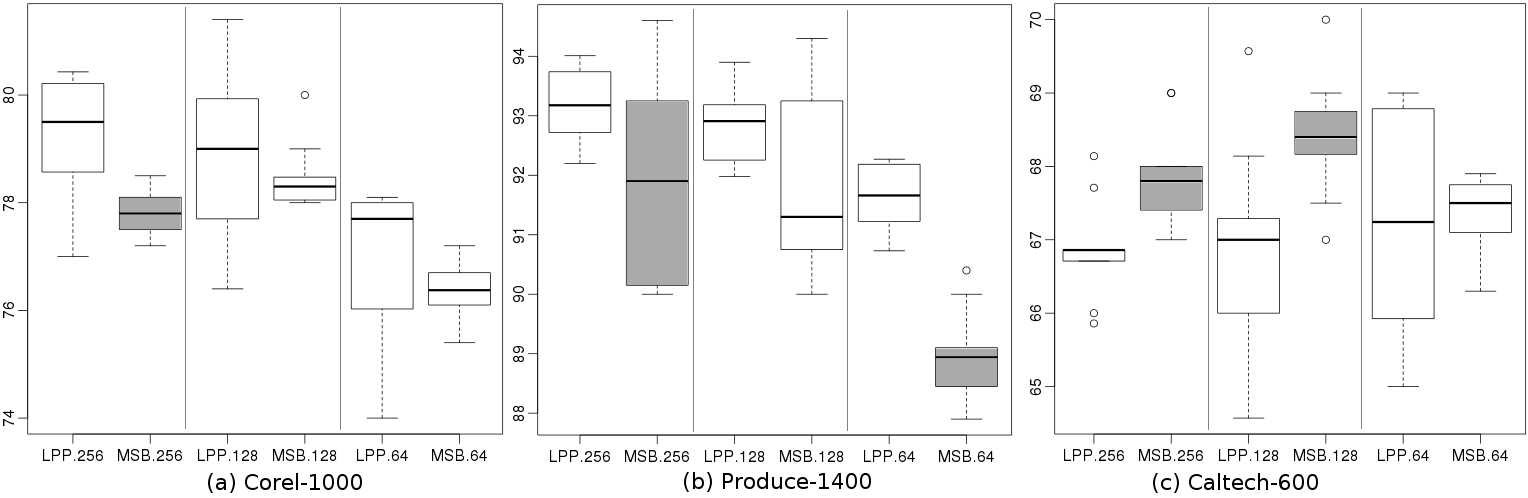
\includegraphics[width=\linewidth]{\detokenize{figuras/quantizacao/fig_results_individual_boxplotMSBLPP.png}}
  \end{center}
  \caption[Resultados de acurácia para os método MSB (quantização), LPP (redução de dimensionalidade) e BIC (extração de características). A comparação do LPP versus MSB foi realizada com a mesma dimensionalidade. Os boxplots em cinza correspondem às significâncias estatísticas com $p < 0.01$ quando comparado a acurácia de 256 cores.]{Resultados de acurácia para os método MSB (quantização), LPP (redução de dimensionalidade) e BIC (extração de características). A comparação do LPP versus MSB foi realizada com a mesma dimensionalidade. Os boxplots em cinza correspondem às significâncias estatísticas com $p < 0.01$ quando comparado a acurácia de 256 cores. \\ \textit{Fonte:~\cite{Ponti2016}.}}
  \label{fig:quant:boxplotMSBLPP}
\end{figure}

O número de dimensões de um vetor resultante de apenas um método de extração de características pode ser considerado baixo. É comum a extração de diversos descritores para uma determinada situação, considerando que normalmente não é claro qual método deveria ser utilizado em cada caso. Por conta disso, os próximos experimentos foram realizados a partir da concatenação de tais características. O objetivo destes experimentos é verificar se a concatenação de todos os descritores pode melhorar os resultados de acurácia. Além disso, comparar os resultados com os experimentos anteriores, afim de verificar se a quantização pode ser uma alternativa à redução da dimensionalidade com métodos convencionais (LPP, neste caso). A melhor configuração encontrada com os experimentos anteriores, entre tamanho do vetor e acurácia, foi utilizando 128 e 64 cores.

A redução do número de cores influencia a dimensionalidade original $D$. O número de características em relação ao número de cores, concatenando todos os vetores resultantes dos métodos de extração de características, é: 256 cores -- 2310 características; 128 cores -- 1160 características; 64 cores -- 582 características; 32 cores --- 294 características; e 16 cores -- 150 características.

Primeiramente, as imagens foram convertidas para escala de cinza e mantidas com 256 cores. Essas imagens foram descritas por todos os métodos de extração e suas características concatenadas em um vetor com dimensão original $D=2310$. A redução de dimensionalidade com LPP foi realizada para $d$ = 1160, 582, 294 e 150. Ou seja, produzindo vetores com o mesmo tamanho dos obtidos apenas com a quantização como método de redução da dimensionalidade. A Figura \ref{fig:quant:resultsFull} mostra os resultados utilizando LPP para as três bases de imagens. Note que o método de quantização MSB resultou em acurácias melhores que os outros métodos.

\begin{figure}[!htbp]
  \begin{center}
    \centering
    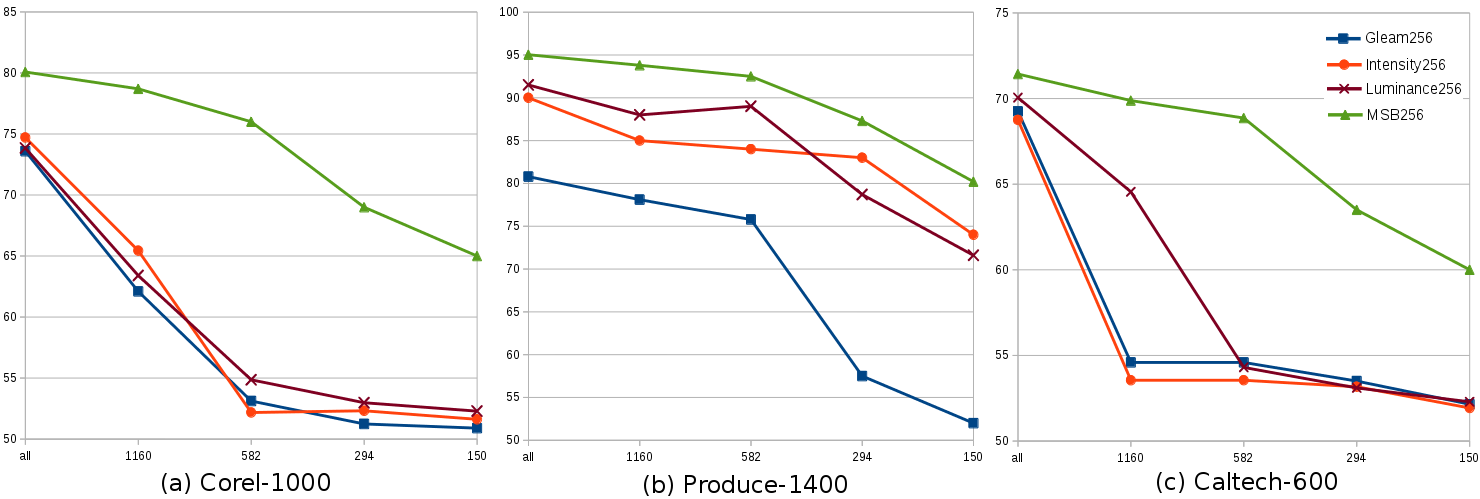
\includegraphics[width=\linewidth]{\detokenize{figuras/quantizacao/fig_results_full.png}}
  \end{center}
  \caption[Comparação da acurácia alcançada com diferentes métodos de quantização: \emph{Gleam}, \emph{Intensidade'}, \emph{Luminância'} e MSB. Inicialmente as imagens foram convertidas para escala de cinza com esses quatro métodos e foram dadas como entrada para todos os métodos de extração. O vetor de características resultante com $D=2310$ sofreu então redução da dimensionalidade com o método LPP para $d = 1160$, $582$, $294$ e $150$.]{Comparação da acurácia alcançada com diferentes métodos de quantização: \emph{Gleam}, \emph{Intensidade'}, \emph{Luminância'} e MSB. Inicialmente as imagens foram convertidas para escala de cinza com esses quatro métodos e foram dadas como entrada para todos os métodos de extração. O vetor de características resultante com $D=2310$ sofreu então redução da dimensionalidade com o método LPP para $d = 1160$, $582$, $294$ e $150$. \\ \textit{Fonte:~\cite{Ponti2016}.}}
  \label{fig:quant:resultsFull}
\end{figure}

A utilização de todos os vetores concatenados melhorou a acurácia em relação ao melhor descritor individual. A Figura \ref{fig:quant:resultsFullBoxplot} apresenta a comparação do espaço original com LPP e MSB para redução da dimensionalidade. Os testes estatísticos ANOVA e o de Tukey foram realizados utilizando $\alpha = 0.01$ como nível de significância. Os resultados que não mudaram significativamente as acurácias foram: MSB com 582 características para a base de dados \emph{Corel}; e \emph{MSB} com 1160 para as três bases. O resultado de piora significativa foi para 32 cores com a base de imagens \textit{Produce}. Dados tais resultados, utilizar 64 cores é apontado como uma boa escolha do parâmetro de quantização.

\begin{figure}[!htbp]
  \begin{center}
    \centering
    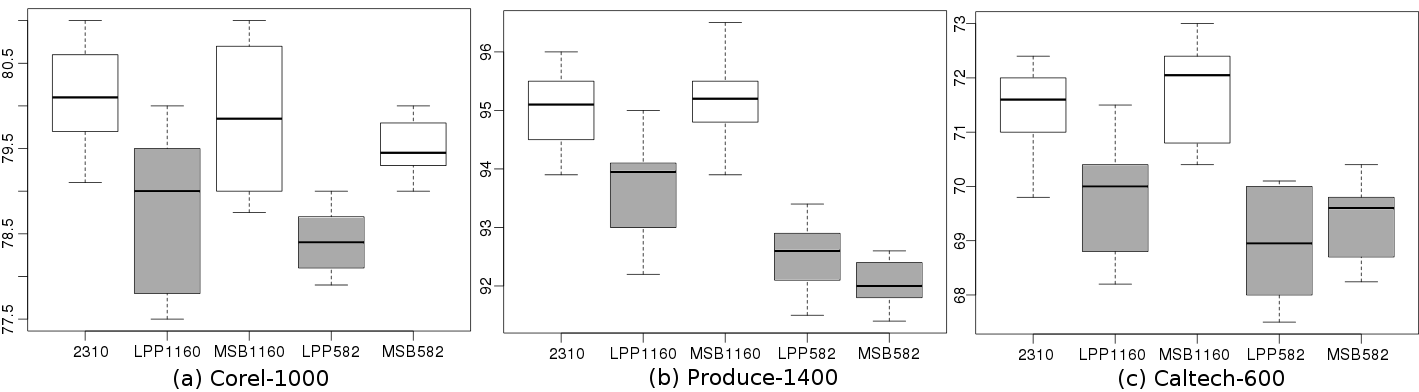
\includegraphics[width=\linewidth]{\detokenize{figuras/quantizacao/fig_results_full_boxplot.png}}
  \end{center}
  \caption[Comparação da acurácia com o uso da projeção LPP e o método MSB para quantização das imagens com o objetivo de redução de dimensionalidade.]{Comparação da acurácia com o uso da projeção LPP e o método MSB para quantização das imagens com o objetivo de redução de dimensionalidade. \\ \textit{Fonte:~\cite{Ponti2016}.}}
  \label{fig:quant:resultsFullBoxplot}
\end{figure}

Os resultados indicam que a quantização pode ser utilizada como redução da dimensão de dados visuais, especialmente utilizando 128 e 64 cores. Como outro experimento, a Figura \ref{fig:quant:fullLPP} mostra as acurácias resultantes da aplicação do LPP sob o vetor obtido após a quantização com MSB utilizando 256 e 64 cores ($d=2310$ e $d=582$, respectivamente). É interessante notar que as projeções LPP em geral foram melhores com as imagens quantizadas em 64 cores com MSB ao invés da original em 256. A razão para isso deve estar no fato da quantização remover informações confusas: ela simplifica as imagens de forma que as cores restantes possam melhor descrever uma certa classe.

\begin{figure}[!htbp]
  \begin{center}
    \centering
    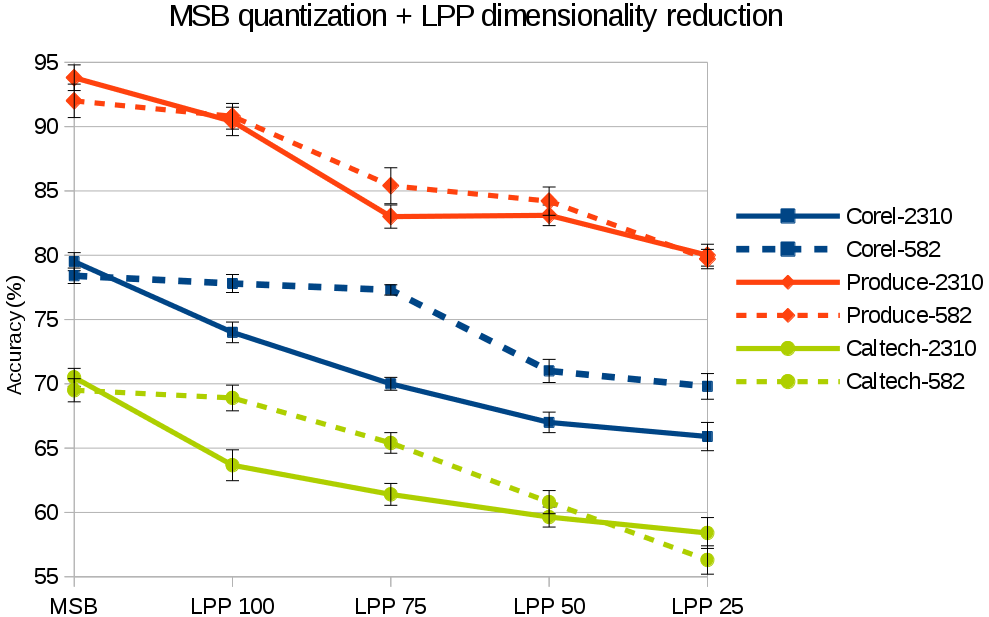
\includegraphics[width=0.6\linewidth]{\detokenize{figuras/quantizacao/fig_results_full_LPP}}
  \end{center}
  \caption[Resultados para a projeção do LPP sobre o espaço de características produzido pelo método de quantização MSB utilizando 256 ($d = 2310$) e 64 cores ($d=582$)]{Resultados para a projeção do LPP sobre o espaço de características produzido pelo método de quantização MSB utilizando 256 ($d = 2310$) e 64 cores ($d=582$)\\ \textit{Fonte:~\cite{Ponti2016}.}}
  \label{fig:quant:fullLPP}
\end{figure}


\section{Considerações Finais}

O vetor concatenado com todos os descritores possui $9C + 6$ dimensões, onde $C$ é o número de cores da imagem de entrada. O tempo de execução para a extração de todas as características é $f(N) = 42N + 6C^2$, onde $N$ é o número de pixels. Para cada imagem são necessárias $D^2 + kD + d^2$ operações para computar o vetor reduzido com LPP, onde $D$ é o tamanho do vetor original, $d$ o tamanho do vetor de saída e $k$ é o número de vizinhos utilizados no algoritmo.

Ao comparar o uso da quantização com a utilização de métodos mais complexos para a redução da dimensionalidade, esse processamento permite uma redução significante, enquanto normalmente preserva ou melhora a acurácia do sistema. Independente da utilização de um método de seleção de características, ao escolher um método de quantização apropriado e seus parâmetros é possível reduzir a dimensionalidade e acelerar computacionalmente as etapas que precedem o reconhecimento de imagens. Considere o seguinte exemplo: 100 imagens com 256 cores demandam 231.6 milhões de instruções para extrair as características e reduzir o vetor utilizando o método LPP (com $k = 10$ e $d = 50$). Se ao invés disso, fossem utilizadas 64 cores, esse número cairia para 58.7 milhões, o que corresponde a uma redução de 74,6\%.
